\documentclass[conference]{IEEEtran}
% Some/most Computer Society conferences require the compsoc mode option,
% but others may want the standard conference format.


% *** CITATION PACKAGES ***
% 
\ifCLASSOPTIONcompsoc
% IEEE Computer Society needs nocompress option
% requires cite.sty v4.0 or later (November 2003)
\usepackage[nocompress]{cite}
\else
% normal IEEE
\usepackage{cite}
\fi
% cite.sty was written by Donald Arseneau
% V1.6 and later of IEEEtran pre-defines the format of the cite.sty package
% \cite{} output to follow that of the IEEE. Loading the cite package will
% result in citation numbers being automatically sorted and properly
% "compressed/ranged". e.g., [1], [9], [2], [7], [5], [6] without using
% cite.sty will become [1], [2], [5]--[7], [9] using cite.sty. cite.sty's
% \cite will automatically add leading space, if needed. Use cite.sty's
% noadjust option (cite.sty V3.8 and later) if you want to turn this off
% such as if a citation ever needs to be enclosed in parenthesis.
% cite.sty is already installed on most LaTeX systems. Be sure and use
% version 5.0 (2009-03-20) and later if using hyperref.sty.
% The latest version can be obtained at:
% http://www.ctan.org/pkg/cite
% The documentation is contained in the cite.sty file itself.
% 
% Note that some packages require special options to format as the Computer
% Society requires. In particular, Computer Society  papers do not use
% compressed citation ranges as is done in typical IEEE papers
% (e.g., [1]-[4]). Instead, they list every citation separately in order
% (e.g., [1], [2], [3], [4]). To get the latter we need to load the cite
% package with the nocompress option which is supported by cite.sty v4.0
% and later.




\usepackage[pdftex]{graphicx}
\graphicspath{{./png/}{./eps/}}
\DeclareGraphicsExtensions{.pdf,.jpeg,.png,.eps}

% *** GRAPHICS RELATED PACKAGES ***
% 
\ifCLASSINFOpdf
% \usepackage[pdftex]{graphicx}
% declare the path(s) where your graphic files are
% \graphicspath{{../pdf/}{../jpeg/}}
% and their extensions so you won't have to specify these with
% every instance of \includegraphics
%\DeclareGraphicsExtensions{.pdf,.jpeg,.png}
\else
% or other class option (dvipsone, dvipdf, if not using dvips). graphicx
% will default to the driver specified in the system graphics.cfg if no
% driver is specified.
% \usepackage[dvips]{graphicx}
% declare the path(s) where your graphic files are
% \graphicspath{{../eps/}}
% and their extensions so you won't have to specify these with
% every instance of \includegraphics
% \DeclareGraphicsExtensions{.eps}
\fi
% graphicx was written by David Carlisle and Sebastian Rahtz. It is
% required if you want graphics, photos, etc. graphicx.sty is already
% installed on most LaTeX systems. The latest version and documentation
% can be obtained at: 
% http://www.ctan.org/pkg/graphicx
% Another good source of documentation is "Using Imported Graphics in
% LaTeX2e" by Keith Reckdahl which can be found at:
% http://www.ctan.org/pkg/epslatex
% 
% latex, and pdflatex in dvi mode, support graphics in encapsulated
% postscript (.eps) format. pdflatex in pdf mode supports graphics
% in .pdf, .jpeg, .png and .mps (metapost) formats. Users should ensure
% that all non-photo figures use a vector format (.eps, .pdf, .mps) and
% not a bitmapped formats (.jpeg, .png). The IEEE frowns on bitmapped formats
% which can result in "jaggedy"/blurry rendering of lines and letters as
% well as large increases in file sizes.
% 
% You can find documentation about the pdfTeX application at:
% http://www.tug.org/applications/pdftex


% *** MATH PACKAGES ***
\usepackage{amsmath}
\interdisplaylinepenalty=2500

% *** SPECIALIZED LIST PACKAGES ***
% 





% *** ALIGNMENT PACKAGES ***
% 
% \usepackage{array}
% Frank Mittelbach's and David Carlisle's array.sty patches and improves
% the standard LaTeX2e array and tabular environments to provide better
% appearance and additional user controls. As the default LaTeX2e table
% generation code is lacking to the point of almost being broken with
% respect to the quality of the end results, all users are strongly
% advised to use an enhanced (at the very least that provided by array.sty)
% set of table tools. array.sty is already installed on most systems. The
% latest version and documentation can be obtained at:
% http://www.ctan.org/pkg/array

\hyphenation{op-tical net-works semi-conduc-tor}

\begin{document}
\title{A Proposal for an Intuitionistic Fuzzy Inference System}


\author{\IEEEauthorblockN{Amaury Hernandez-Aguila, Mario
    Garcia-Valdez, Oscar Castillo}
  \IEEEauthorblockA{Tijuana Institute of Technology\\
    Division of Graduate Studies and Graduates\\
    Tijuana, Mexico\\
    Email: \{amherag,mario,ocastillo\}@tectijuana.edu.mx}}

\maketitle

\begin{abstract}
The concepts of intuitionistic membership, and intuitionistic center of
area are proposed in this work, in order to propose a novel method for
implementing an intuitionistic fuzzy inference system. The proposed
method was implemented and compared against type-1 fuzzy inference
systems and interval Type-2 fuzzy inference systems, with uncertain
means and uncertain standard deviations, by using the
Mackey-Glass time series benchmark. A genetic algorithm was used to
optimize the parameters of each of the methods being compared, and the
results show that the intuitionistic fuzzy inference system performs
better than the other methods.
\end{abstract}

\IEEEpeerreviewmaketitle



\section{Introduction}

Fuzzy sets were created as an extension to traditional sets, with
uncertainty in mind, by L. A. Zadeh in 1965 \cite{zadeh1965fuzzy}. This uncertainty allows an
element to be associated with a grade of membership that indicates
how much that element belongs to a set, i.e., instead of
belonging to a set (true, or 1), or not belonging (false, or 0),
such element can belong in a grade from 0 to 1, and this is known as
fuzzy logic \cite{klir1995fuzzy}.

A derivation of logical conclusions can be performed by using premises
that are assumed to be true, and this is known as inference, in
traditional logic. The same
technique can be extended to use fuzzy premises. In this case, all the
premises hold a grade of truthiness, and a fuzzy conclusion is derived
from the process. A popular method for performing such fuzzy inferences is a
Mamdani Fuzzy Inference System (FIS) \cite{mamdani1975experiment},
where the inputs are associated with fuzzy sets, and the outputs are
fuzzy sets themselves, which can be converted to crisp numbers
(this process is usually called \textit{defuzzification}). Other types of
fuzzy inference engines exist, such as Takagi-Sugeno-Kang  (TSK)
\cite{takagi1985fuzzy} and Tsukamoto \cite{tsukamoto1979approach}.

Fuzzy sets were initially criticized because they were said to
not be able to appropriately represent uncertainty. This problem was
addressed by L. A. Zadeh in 1975 \cite{zadeh1975concept} by creating the
concept of Type-2 Fuzzy Sets (T2-FS). This extension to type-1 fuzzy sets allowed the creation of
type-2 fuzzy inference systems (T2-FIS) \cite{mendel2002type}, and those systems that used the
traditional fuzzy sets are now called Type-1 Fuzzy Inference Systems
(T1-FIS). T2-FIS have been proved to work better than T1-FIS in many
situations, often problems that involve high levels of uncertainty, such as
noisy data.

Another extension to fuzzy sets, called Intuitionistic Fuzzy Sets
(IFS), was proposed by K. T. Atanassov
\cite{atanassov1986intuitionistic}. This extension adds the concepts
of indeterminacy and non-membership to traditional fuzzy sets. In
traditional fuzzy sets, the non-membership of an element is always the
complement of the membership, but in an IFS, the non-membership can be
represented by lower values (a deeper explanation of IFS is given in
Section \ref{preliminaries}). Whenever the sum of the membership and
the non-membership is less than 1, indeterminacy emerges, which
represents the grade of uncertainty of an element of being or not
being a member of a given set, with certain grade of membership. The
concept of indeterminacy allows an expression such as ``This is
somewhat tall, although I'm not very sure about my opinion.''

The use of IFSs in a traditional FIS should enable the handling of more
uncertainty, and one could prefer an Intuitionistic FIS (IFIS) to obtain
better accuracies without sacrificing time performance, as
inferences in a T2-FIS are very time consuming compared to a
T1-FIS. This is a consequence of the complex type
reducing procedure that is involved in the defuzzification stage in a
T2-FIS \cite{mendel2001uncertain}. Several improvements to the
algorithms involved in the inference process in a T2-FIS have been proposed
to alleviate this problem, such as the Karnik-Mendel algorithm
\cite{wu2009enhanced} and shadowed sets
\cite{pedrycz1998shadowed}. Nevertheless, a T2-FIS is usually several
times slower than a T1-FIS. Because of this time performance impact,
many works that require handling more uncertainty than a T1-FIS
use a particular case of T2-FIS, the Interval T2-FIS (IT2-FIS)
\cite{mendel2006interval}, which is faster than a general T2-FIS. A Type-1
Intuitionistic FIS (T1-IFIS) should perform better than a T1-FIS in terms
of accuracy (in problems involving data with high levels of
uncertainty), and should be faster than a T2-FIS. Furthermore, IFSs
can be implemented as part of a T2-FIS, giving as a result a T2-IFIS.

This work proposes a method to implement IFSs in a Mamdani FIS to
obtain a Mamdani IFIS, and presents results that prove the method as a
viable design to implement an effective IFIS. The reader can find
related works in Section \ref{related-work}. Some preliminaries are
explained in Section \ref{preliminaries} in order to better comprehend
the proposed method in Section \ref{proposed-method}. Experiments were
conducted to prove the viability of the proposed method, and they are
explained in Section \ref{experiments}. The results of the conducted
experiments are shown and explained in Section \ref{results}, and a
conclusion about the results is presented in Section
\ref{conclusion}. Finally, a description of the future work can be
found in Section \ref{future-work}.


%What is a intuitionistic fuzzy set? \cite{atanassov1986intuitionistic}
%\cite{atanassov2003intuitionistic} \cite {despi2013generalised}

% (Mario): 
% Más que definir los elementos, mejor justificar el motivo de la propuesta
% al parecer es por que Type-2 is time-consuming  
%   --(Amaury)
%% -- Sí y no. Hacerlo intuicionista le añade el concepto de
%% indeterminación. No es un reemplazo del tipo-2, en realidad le
%% añade cosas. Ahora, sí es parte de la justificación, ya que alguien
%% puede optar por usar un tipo-1 intuicionista en lugar de un tipo-2
%% por intervalos, por ejemplo, porque puede ser que gane performance
%% parecido al de un tipo-2, sin tener el time-consuming de un
%% tipo-2. Igual puede haber un tipo-2 intuicionista.


% Esto si:
% What is a intuitionistic fuzzy set 
% Y después justificar, debido a esto, proponemos un FIS intucionista
% Después lo clasico de como esta dividido el trabajo
%% (Amaury): Ok! Voy a dar una descripción básica, ya que en la
%% sección de preliminares es donde explico a fondo

\section{Related Work}
\label{related-work}

Application of intuitionistic fuzzy sets, bacillus colonies
recognition \cite{davarzani2013novel}

Alpha cut \cite{sharma2011cut} \cite{sharma2011cutgroups}

intuitionistic inference engine \cite{cornelis2001compositional} %Que
                                %diferencias hay?
%% (Amaury): oh, sí voy a poner las diferencias. Nomás puse todo esto
%% para acordarme :D

implementation of a ifis, castillo \cite{castillo2007intuitionistic}
% Por?  
%% (A): Porque es lo más cercano a un FIS mamdani intuicionista. al
%% menos de lo que encontré.

more inference \cite{bustince1995method}

centroid of a type-2 fuzzy-set \cite{karnik2001centroid} %Por?
%% Porque yo propongo una fórmula para calcular centroide de un IFS, y
%% como la competencia de un IFS sería un fuzzy set tipo 2, iba a
%% hablar un poco de eso

and even more inference \cite{marinov2005method}

Intuitionistic control washing machines \cite{akram2014intuitionistic}

\section{Preliminaries}
\label{preliminaries}

Define in more detail intuitionistic fuzzy sets. 

Formulas and basic explanation (below) \cite{atanassov2013intuitionistic}

% intuitionistic fuzzy set
\begin{equation}
  A^{*} = \{\langle x, \mu _{A} (x), \nu _{A} (x) \rangle | x \in E\}
\end{equation}

% intuitionistic interval
\begin{equation}
  \label{intuitionistic-interval}
  0 \leq \mu_{A}(x) + \nu_{A}(x) \leq 1
\end{equation}

% every ordinary fuzzy set has the form
\begin{equation}
  \label{ifs-form}
  \{ \langle x, \mu_{A}(x), 1 - \mu_{A}(x) \rangle | x \in E \}
\end{equation}

% if
\begin{equation}
  \label{fs-as-ifs-if}
  \pi_{A}(x) = 1 - \mu_{A}(x) - \nu_{A}(x)
\end{equation}

\section{Proposed Method}
\label{proposed-method}
%(Mario)Is a Method? Extension? Implementation?
%% (A): No lo había pensado en realidad. Es que siempre le llamo
%% Proposed Method jajajaaj. Aunque creooo que sí es un método. Es un
%% método para hacer un sistema de inferencia difusa con conjuntos
%% difusos intuicionistas
The method, for now, consists on the procedures and elements
necessary to construct a basic Intuitionistic Fuzzy Inference System
(IFIS). %(Mario)Por que basic?
%% (A): Basic porque no añado que puedas poner OR en las reglas, no
%% pongo otros métodos de defuzzificación, no pongo más funciones de
%% membresía (triangulares, etc.). Explicaré eso (y)
%(Mario)Tal vez enumerarlas? cuales procedures son?
%% (A): Los procedures son los que están en el diagramita, y las
%% explico abajo. Aun así las enumero?
An implementation was completed in order to make comparisons against
classic Fuzzy Inference Systems (FISs), such as Type-1 FIS, Interval
Type-2 and General Type-2 FIS, and prove that
the design was viable and able to contribute to better results than
the classic FISs.
%(Mario)Es el proposito del diseño comparar? Creo que puedes decir mejor algo como:
%In order to assess the advantage of our proposal in terms of X
%a comparassion with  Type-1 FIS, Interval Type-2 and General Type-2 FIS,
%is presented.

%% (A): Ok, me gusta.

%que se vea que tiene su merito propio, y lo comparamos para
%evaluar y comprobar su viabilidad
%Lo de Design me ocasiona ruido, parece que fuera una implementación
%Si no lo es, tal vez se puede decir algo como:
%The proposed method was implemented in order to make.

%% (A): Ya lo cambié al principio, pero el design en "prove that the
%% design was viable" no sé si cambiarlo

In many works, intuitionistic fuzzy sets (IFSs) are constructed manualy,
by interviewing experts who assign memberships and
non-memberships to each of the values of a set (such as in %to each of the members of a set?
\cite{davarzani2013novel}). This work proposes a convenient way of
creating an IFS, imitating many systems that use Gaussian
membership functions (MFs) to facilitate an expert the representation of a
fuzzy interpretation. An example of an IFS is depicted in
Figure \ref{fs-as-ifs}. This IFS represents a classic fuzzy set, as it
satisfies (\ref{ifs-form}) and (\ref{fs-as-ifs-if}), by representing
the MF as the red line, and the non-membership
function (NMF) as the blue line. In order to contruct the NMF, one has
to rotate a normal Gaussian MF by 180˚, and this can be seen as the
complement of the fuzzy set corresponding to a Gaussian MF.
%(Mario)Al parecer lo que se está presentando es una manera automatizada de 
% hacer IFSs? Si  es así, es más facil presentarlo
%% Si se hacen automatizadamente para poder compararlo con el tipo-1 y
%% tipo-2, pero no es el objetivo del trabajo.

\begin{figure}[!t]
  \centering
  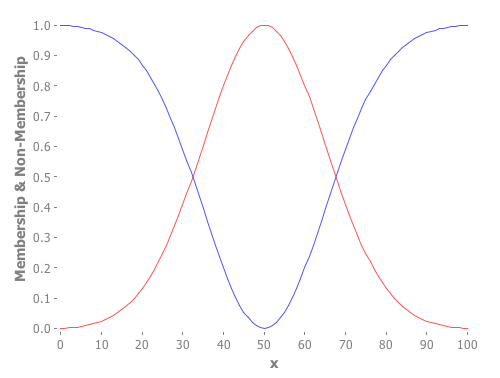
\includegraphics[width=2.5in]{fs-as-ifs}
  \caption{Classic Fuzzy Set Represented as an Intuitionistic Fuzzy Set}
  \label{fs-as-ifs}
\end{figure}

Two convenient ways of modifying a NMF and also
satisfying (\ref{intuitionistic-interval}) are the following: 1) setting
the mean and the standard deviation of the Gaussian functions to be
the same, and only vary the \textit{height} of the NMF,
as is depicted in Figure \ref{ifs}; and 2) setting different means and
standard deviations of the Gaussian membership and non-membership
functions, while keeping the \textit{height} of the MF equal
to $h_{mf} = 1 - h_{nmf}$, as this ensures that
(\ref{intuitionistic-interval}) is satisfied. An example of the latter
case is shown in Figure \ref{ifs-diff-mu-sd}. To clarify, the \textit{height}
of the MF ($h_{mf}$) of an IFS is equal to $max(\mu(x))$, and the
\textit{height} of the NMF ($h_{nmf}$) of an IFS is equal to $max(\nu(x))$.

\begin{figure}[!t]
  \centering
  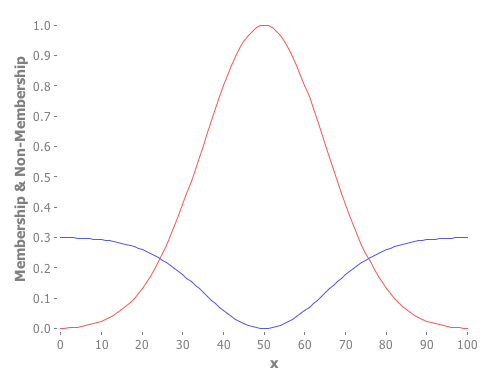
\includegraphics[width=2.5in]{ifs}
  \caption{An Example of an Intuitionistic Fuzzy Set - Same Mean and SD}
  \label{ifs}
\end{figure}

\begin{figure}[!t]
  \centering
  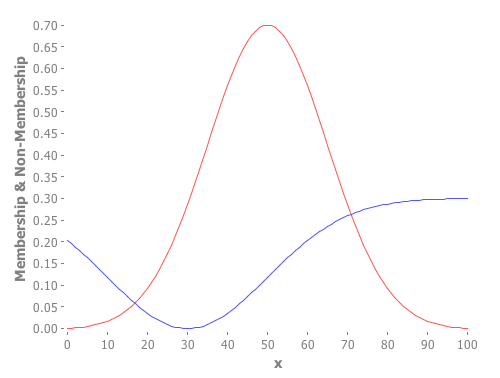
\includegraphics[width=2.5in]{ifs-diff-mu-sd}
  \caption{An Example of an Intuitionistic Fuzzy Set - Different Mean
    and SD}
  \label{ifs-diff-mu-sd}
\end{figure}

The first step of the inference process in a classic FIS (a flow chart
for the process in an IFIS is given in Figure \ref{flow-chart}) is to
determine what grade of membership corresponds to a given input, given a set of
%(Mario)determine what particular membership function corresponds to a 
% given input, given a set of 
%% (A): Es grade of membership, perdón. De hecho hay ese error en
%% otras partes, tengo que cambiarlo.
MFs. This is straightforward in a classic FIS, as the
membership to each input is already established in the membership
fuzzy set. For an IFIS, this work proposes a method to determine a
membership given a MF and a NMF,
which is described in (\ref{imembership}), and receives the name of
$i\mu$ (intuitionistic membership). %(Mario)Creo que este podría ser
                                %el titulo
%% (A): Para poder hacer un FIS intuicionista, necesité el
%% intuitionistic membership y el intuitionistic center of area. Cómo
%% propone el título?

\begin{figure}[!t]
  \centering
  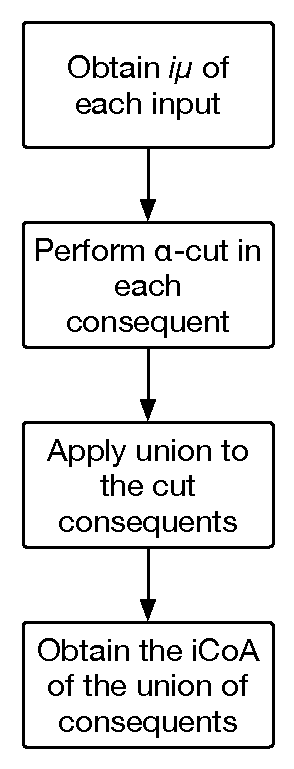
\includegraphics[height=2.5in]{proposed-method-flow-chart}
  \caption{Proposed Method Flow Chart}
  \label{flow-chart}
\end{figure}

% i-membership
\begin{equation}
  \label{imembership}
  i\mu_{A}(x) = (\nu_{A}(x) + \mu_{A}(x))\mu_{A}(x)
\end{equation}

A comparison of a MF (red line) against an intuitionistic
membership function (blueline) is shown in Figure
\ref{if-membership}. The parameters for both the MF and NMF are $\mu =
50$ and $SD = 15$, but the \textit{height} for the NMF is set at \textit{0.5}. This
results in an intuitionistic MF that appears to have the same mean,
but a smaller standard deviation. A more elaborated example is shown
in Figure \ref{if-membership-drastic}, where the parameters of the MF
are $\mu = 50$, $SD = 15$ and $h = 0.8$, and the parameters of the NMF
are $\mu = 30$, $SD = 20$ and $h = 0.2$. As can be noted, the
indeterminacy ($\pi$) is high in this example, which results in a
smaller $SD$ for the intuitionistic MF. Moreover, the difference in
means and standard deviations generates a change of the mean for the
intuitionistic MF.

\begin{figure}[!t]
  \centering
  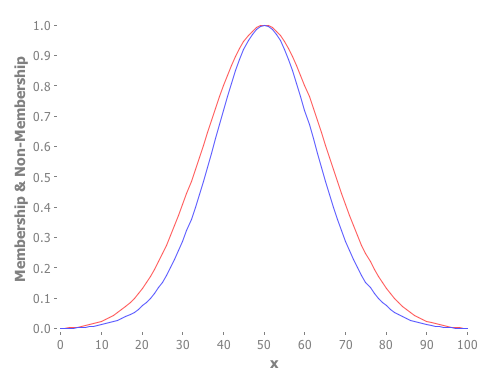
\includegraphics[width=2.5in]{if-membership}
  \caption{Comparison of $\mu(x)$ Against $i\mu(x)$}
  \label{if-membership}
\end{figure}

\begin{figure}[!t]
  \centering
  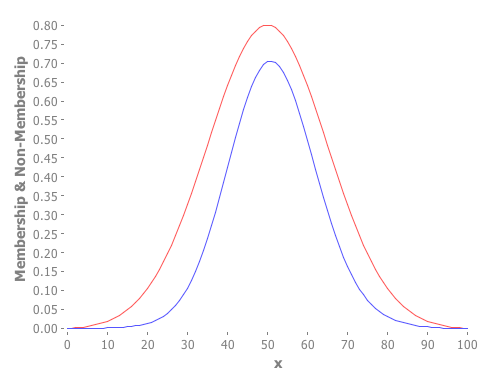
\includegraphics[width=2.5in]{if-membership-drastic}
  \caption{Comparison of $\mu(x)$ Against $i\mu(x)$ With More Indeterminism}
  \label{if-membership-drastic}
\end{figure}

The next step in the inference process is to perform an $\alpha$-cut % (Mario)
La del FIS? aclaralo on the associated consequents to the antecedents that are
activated by the inputs. In a classic FIS, this process is straightforward, as
the memeberships in a fuzzy set representing a consequent are ``cut'' by
following (\ref{alpha-cut}) for every element in a fuzzy set representing a
consequent. In an intuitionistic MF, one can follow the same procedure in order
to obtain the $\alpha$-cut in the MF part, but to obtain the $\alpha$-cut in
the NMF, (\ref{nmf-alpha-cut}) must be followed. In (\ref{nmf-alpha-cut}), the
counterintuitive part is that one has to find the corresponding $\nu$ for a
given $\mu_{\alpha}$. An example of an $\alpha$-cut, with $\mu_{\alpha} = 0.6$,
is depicted in Figure \ref{alpha-cut-example}.

\begin{equation}
  \label{alpha-cut}
  \alpha(\mu (x),\mu_{\alpha}) =
  \begin{cases}
    \mu (x), & \text{if}\ \mu (x) \leq \mu_{alpha}  \\
    \mu_{\alpha}, & \text{otherwise}
  \end{cases}
\end{equation}

\begin{equation}
  \label{nmf-alpha-cut}
  \alpha_{NMF}(\nu (x),\mu_{\alpha}) =
  \begin{cases}
    \nu (x), & \text{if}\ \nu (x) \geq \nu (\mu_{alpha})  \\
    \nu (\mu_{alpha}), & \text{otherwise}
  \end{cases}
\end{equation}

\begin{figure}[!t]
  \centering
  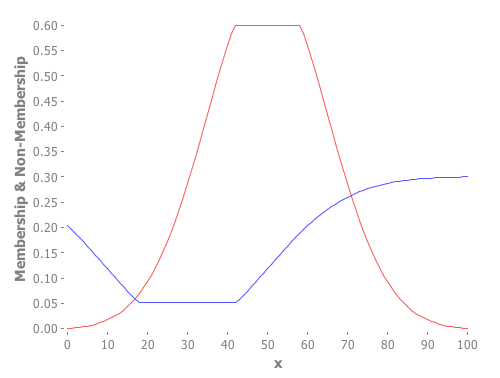
\includegraphics[width=2.5in]{alpha-cut}
  \caption{$\alpha$-cut of an Intuitionistic Fuzzy Set}
  \label{alpha-cut-example}
\end{figure}

After performing every necessary $\alpha$-cut, one has to apply the
union operator over every resulting fuzzy set, in order to aggregate
the weights of all the consequents. The union operator is defined by
K. Atanassov \cite{atanassov2013intuitionistic}, for every two IFSs A
and B, as in (\ref{union-operator}). An example of an union of three
IFSs is shown in Figure (\ref{ifs-union}).

\begin{equation}
  \label{union-operator}
  \begin{aligned}
    A \cup B  = &\{ \langle x, max(\mu_{A} (x), \mu_{B} (x)),\\
    &\quad min(\nu_{A} (x), \nu_{B} (x)) \rangle | x \in E \}
\end{aligned}
\end{equation}

\begin{figure}[!t]
  \centering
  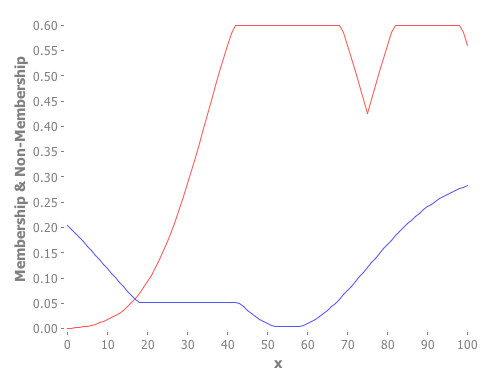
\includegraphics[width=2.5in]{ifs-union}
  \caption{Union of Three $\alpha$-cut Intuitionistic Fuzzy Sets}
  \label{ifs-union}
\end{figure}

Finally, one has to defuzzify the aggregation of the $\alpha$-cut 
consequents, in order to obtain a crisp number that represents
it. There are a number of methods that can be used to defuzzify a
% Aclara que en los tipo Mamdany %% (A): ahhhhh cierto, cierto
fuzzy set, but the most frequently found in the literature is the
Center of Area (CoA), or simply centroid. One can obtain the centroid
of a classic fuzzy set A by using (\ref{center-of-area}). For an
IFS, one can use the concept of intuitionistic membership ($i\mu$) and
extend (\ref{center-of-area}) to obtain (\ref{if-coa}). By
substituting $(\mu(x_{i}) + \nu(x_{i}))$ by $i\mu_{A}$, one arrives at
(\ref{if-coa-simplified}), which is a simplification of (\ref{if-coa}).

% CoA
\begin{equation}
  \label{center-of-area}
  A_{CoA} = \dfrac{\sum_{i=1}^{N} \mu(x_{i})
    x_{i}}{\sum_{i=1}^{N} \mu(x_{i})}
\end{equation}

%iCoA
\begin{equation}
  \label{if-coa}
  A_{iCoA} = \dfrac{\sum_{i=1}^{N} (\mu(x_{i}) + \nu(x_{i})) \mu(x_{i})
    x_{i}}{\sum_{i=1}^{N} (\mu(x_{i}) + \nu(x_{i})) \mu(x_{i})}
\end{equation}

%iCoA contracted
\begin{equation}
  \label{if-coa-simplified}
  A_{iCoA} = \dfrac{\sum_{i=1}^{N} i\mu_{A}(x) x_{i}}{\sum_{i=1}^{N}
    i\mu_{A}(x)}
\end{equation}

Figure \ref{if-coa-vs-coa} shows the plot of the defuzzification of
several IFSs with $CoA$ (red line) and $iCoA$ (blue line), with means set
from 0 to 100 for the MF, and -20 to 80 for the NMF, and standard
deviations of 15 for the MF, and 20 for the NMF.

\begin{figure}[!t]
  \centering
  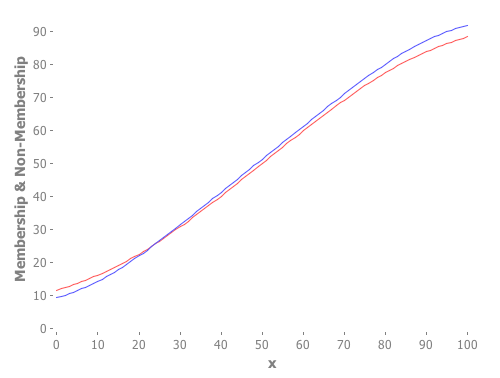
\includegraphics[width=2.5in]{if-coa-vs-coa}
  \caption{Comparison of $CoA_{A_{i}}$ Against $iCoA_{A_{i}}$}
  \label{if-coa-vs-coa}
\end{figure}

\section{Experiments}
\label{experiments}

The purpose of the experiments in this work is to demonstrate that the
proposed method is viable for performing inference using
intuitionistic fuzzy sets instead of classic fuzzy sets, i.e., that
the concepts of intuitionistic membership ($i\mu$) and intuitionistic
center of area ($iCoA$) enable an extension to traditional fuzzy
inference systems to support indeterminacy and non-membership. To
demonstrate this claim, this work presents a series of experiments
where the proposed method is compared against Type-1 Fuzzy Inference
Systems (T1-FISs) and Interval Type-2 Fuzzy Inference Systems
(T2-FISs) with uncertain mean and uncertain standard deviation.

The initial (and ambitious) hypothesis is that a Type-1 Intuitionistic Fuzzy System (T1-IFIS)
should perform better than a T1-FIS, as it can handle both uncertainty
and indeterminacy, and it is unclear if an IFIS should perform better
than a T2-FIS. The experiments presented in this work
cannot prove this statement profoundly, as the results will only be tested for a
single situation, which is the prediction of a subset of the
Mackey-Glass time series.

An implementation of the proposed method was developed using the
programming language Clojure, and it is freely accessible at
https://github.com/amherag/intuitionistic-fis. The T1-FISs and
IT2-FISs were developed using Juzzy \cite{wagner2013juzzy}, which
implements T1-FIS, IT2-FIS and GT2-FIS in Java.

The Mackey-Glass time series benchmark was used in order to compare
the performances of each of the FISs regarding their time series
forecasting capabilities, and a Genetic Algorithm (GA) was
used to optimize each of the FISs, so sub-optimal versions of each of
the systems were used for the comparison.
%M: En esta seccion creo que se

Every FIS uses the following rule base:

\begin{enumerate}
  \item if $t_{0}$ is $A_{1}$ then $p_{t+1}$ is $C_{1}$
  \item if $t_{-6}$ is $A_{2}$ then $p_{t+1}$ is $C_{2}$
  \item if $t_{-12}$ is $A_{3}$ then $p_{t+1}$ is $C_{3}$
  \item if $t_{-18}$ is $A_{4}$ then $p_{t+1}$ is $C_{4}$
\end{enumerate}
where $t_{0}$, $t_{-6}$, $t_{-12}$, and $t_{-18}$ are points in the
Mackey-Glass time series, $t_{0}$ is the present point, $t_{-6}$ is six
points earlier than $t_{0}$, $t_{-12}$ is twelve points earlier, and
$t_{-18}$ is eighteen points earlier. $p_{t+1}$ is the predicted value
for the point $t_{1}$. $A_{1}$, $A_{2}$, $A_{3}$, and $A_{4}$ are
antecedents, and $C_{1}$, $C_{2}$, $C_{3}$, and $C_{4}$ are
consequents.

The dataset consists of 100 data points for training, and 50 data
points for testing. These data points were scaled, such that the
resulting data points range from 0 to 100. The scaling process was
performed by applying (\ref{scaling}) over each of the data points in
the union of the training and testing subsets. The reason behind this
preprocessing is that the implementation of the IFIS works with inputs
ranging from 0 to 100, but the Mackey-Glass time series' data points
range from 0 to about 1.4. This does not alter the measurement of the
error produced by each of the FISs, as the outputs from the FISs are
also scaled from 0 to 100.

\begin{equation}
  \label{scaling}
  S(p) = 100 \frac{p - min(P)}{max(P) - min(P)}
\end{equation}

The search space for the GA consists on eight tuples with the form $\langle
mean, standard deviation \rangle$ for the T1-FIS, $\langle
mean, standard deviation, height \rangle$ for the IFIS, $\langle
mean, standard deviation 1, standard deviation 2 \rangle$ for the
IT2-FIS with uncertain standard deviation, and $\langle
mean 1, mean 2, standard deviation \rangle$ for the IT2-FIS with
uncertain mean, where the means and standard deviations can take
random real numbers from 0 to 100, and the height can take random real
numbers from 0.8 to 1. Each of the individuals in the GA consists on
eight tuples, one for each of the four antecedents and four
consequents in a FIS. The rule base isn't optimized.

Regarding the parameters of the GA, every FIS is optimized for 20
generations, using 100 individuals as the initial population. The
roulette wheel method is used as the selection operator. Five
children are generated each generation and replace the five least
fitted individuals in the population. For the mutation operator, each
individual in the population has a chance of 1\% of suffering an
alteration, which consists on replacing a list of tuples of arbitrary
length from the affected individual with a list of tuples of the same
length from another random individual in the population. Finally, the
crossover operator takes random genetic material from two individuals
and creates a child of the same length as its parents. The genetic
material cannot be repeated, can be of different proportions from each
of the parents, and the original order isn't preserved. For example,
given the individuals $A = <1, 2, 3, 4>$ and $B = <5, 6, 7, 8>$, a
possible child is $C = <8, 1, 7, 5>$. This operator was developed
because it proved by trial and error that it created more diversity in
the children than other operators such as one-point or two-point
crossover.

To obtain the performance of a particular individual, a FIS is created
using the parameters represented by its genetic material. The created
FIS is then evaluated with each of the inputs in the training dataset
(100 sets of four data points: $t_{0}$, $t_{-6}$, $t_{-12}$, and
$t_{-18}$). The outputs (i.e. the 100 predicted values) for each of
the inputs are then scaled from 0 to 100, as was mentioned before, so
a Mean Squared Error (MSE) can be obtained by comparing the predicted values
to the scaled Mackey-Glass' points ($p_{t+1}$). Individuals with lower
MSEs are said to be performing better.

Finally, the better performing individual after the 20 generations in
the GA is evaluated using the training and testing datasets, and the
resulting MSEs are used as the result of one experiment. In total, 60
experiments were performed for the T1-IFIS, 60 for the T1-FIS, 100 for
the IT2-FIS with uncertain mean, and 300 for the IT2-FIS with
uncertain standard deviation.

% Comparisons against juzzy \cite{wagner2013juzzy}

% Compare using Mackey-Glass, 100 training, 50 for testing, because it
% took too much time. Genetic algorithm. Present parameters: mean 0-100,
% sd 30-70, mf 1, nmf 0.8-1.0.

% The rule base.

\section{Results}
\label{results}

The full results (CSV files containing the MSE for each of the
experiments) along with the Clojure source code used to obtain the
data presented in this section can be found on the following public
Github repository: https://github.com/amherag/wcci-2016-a.

Initially, 60 experiments were performed for every FIS, but that
number of experiments didn't provide enough statistical data for the
IT2-FISs in order to make a conclusion. For the IT2-FIS with uncertain
mean, 100 experiments were needed to provide enough statistical data
to conclude what FIS performed better, and for the IT2-FIS with
uncertain standard deviation, 300 experiments were needed. To clarify,
all of the comparisons were against the T1-IFIS.

Table \ref{first-hypothesis-tests-training} summarizes the results obtained
for each of the FISs in the training stage, as well as the t-value
obtained when calculating a Student's t-test. The same structure is
followed in Table \ref{first-hypothesis-tests-testing}, which shows the
results obtained for each of the FISs in the testing stage.

\begin{table}[!t]
  \renewcommand{\arraystretch}{1.3}
  \caption{Hypothesis Tests for the Training Stage, First Experiment}
  \label{first-hypothesis-tests-training}
  \centering
  \begin{tabular}{|c|c|c|c|c|c|}
    \hline
    Method & $\mu_{TR}$ & $SD_{TR}$ & $n$ & t-Value & CI \\
    \hline
    T1-IFIS & 89.50 & 25.36 & 60 &  & \\
    \hline
    T1-FIS & 108.05 & 23.47 & 60 & -4.1584 & > 99.9\% \\
    \hline
    IT2-FIS (\(\mu\)) & 112.56 & 29.16 & 100 & -5.2597 & > 99.9\% \\
    \hline
    IT2-FIS (SD) & 102.31 & 26.08 & 300 & -3.5548 & > 99.9\% \\
    \hline
  \end{tabular}
\end{table}

% con 400
\begin{table}[!t]
  \renewcommand{\arraystretch}{1.3}
  \caption{Hypothesis Tests for the Training Stage, Second Experiment}
  \label{second-hypothesis-tests-training}
  \centering
  \begin{tabular}{|c|c|c|c|c|c|}
    \hline
    Method & $\mu_{TR}$ & $SD_{TR}$ & $n$ & t-Value & CI\\
    \hline
    T1-IFIS & 76.22 & 16.90 & 400 & & \\
    \hline
    T1-FIS & 85.69 & 19.68 & 400 & -7.3013 & > 99.9\% \\
    \hline
    IT2-FIS (\(\mu\)) & 85.93 & 19.12 & 400 & -7.6102 & > 99.9\%\\
    \hline
    IT2-FIS (SD) & 99.78 & 19.04 & 400 & -18.508 & > 99.9\% \\
    \hline
  \end{tabular}
\end{table}

\begin{table}[!t]
  \renewcommand{\arraystretch}{1.3}
  \caption{Hypothesis Tests for the Testing Stage, First Experiment}
  \label{first-hypothesis-tests-testing}
  \centering
  \begin{tabular}{|c|c|c|c|c|c|}
    \hline
    Method & $\mu_{TS}$ & $SD_{TS}$ & $n$ & t-Value & CI \\
    \hline
    T1-IFIS & 160.99 & 65.70 & 60 &  & \\
    \hline
    T1-FIS & 194.97 & 71.97 & 60 & -2.7010 & > 99.2\%\\
    \hline
    IT2-FIS (\(\mu\)) & 192.31 & 105.75 & 100 & -2.3104 & > 97.8\% \\
    \hline
    IT2-FIS (SD) & 178.63 & 99.70 & 300 & -1.7209 & > 91.4\% \\
    \hline
  \end{tabular}
\end{table}


% con 400
\begin{table}[!t]
  \renewcommand{\arraystretch}{1.3}
  \caption{Hypothesis Tests for the Testing Stage, Second Experiment}
  \label{second-hypothesis-tests-testing}
  \centering
  \begin{tabular}{|c|c|c|c|c|c|}
    \hline
    Method & $\mu_{TS}$ & $SD_{TS}$ & $n$ & t-Value & CI\\
    \hline
    T1-IFIS & 139.38 & 95.75 & 400 &  &  \\
    \hline
    T1-FIS & 152.26 & 126.47 & 400 & -1.6239 & > 89.4\% \\
    \hline
    IT2-FIS (\(\mu\)) & 154.37 & 119.92 & 400 & -1.9536 & > 94.8\% \\
    \hline
    IT2-FIS (SD) & 175.04 & 136.91 & 400 & -4.1492 & > 99.9\%\\
    \hline
  \end{tabular}
\end{table}

\section{Conclusion}
\label{conclusion}

As the results in Section \ref{results} demonstrate, the T1-IFIS
outperforms the T1-FIS, IT2-FIS with uncertain mean, and IT2-FIS with
uncertain standard deviation. These results sustain the claim that the
intuitionistic grade of membership ($i\mu$), and the intuitionistic center
of area ($iCoA$), proposed in Section \ref{proposed-method} allows the
creation of a T1-IFIS that can perform better than a classic T1-FIS
and an IT2-FIS.

Several derivative works can result from the ideas presented in this paper. For
example, the proposed T1-IFIS can be tested using several
benchmarks, other than the Mackey-Glass time series. Also, this work
should inspire the creation of Type-2 Intuitionistic Fuzzy Inference
Systems (both the interval and general types).

\section{Future Work}
\label{future-work}

The current implementation of the proposed method lacks a Graphical User
Interface (GUI) where a research can conveniently design an IFIS, such as
Matlab's Type-1 Fuzzy Logic toolbox, or the Type-2 Fuzzy Logic toolbox
developed by J. R. Castro \textit{et al.} \cite{castro2007interval}. The
development of a GUI is planned as a next step, so researchers without
a background in the programming langague Clojure can use the
implementation for their works.

In theory, an implementation of the proposed method should be faster
than T2-FISs, and slower than T1-FISs (although this difference should
be negligible), but the current implementation performs worse, in
terms of time, than a general T2-FIS. This has to be solved in order
to speed up the experiments conducted, and to encourage other
researchers to use the implementation.

\bibliographystyle{IEEEtran}
\bibliography{paper}

\end{document}
